% 
% (c) 2015, Florian Mayer
%
% This document is released under the terms
% of the GNU Free Documentation License
%
% See LICENSE for further information regarding
% this license.
%%

\documentclass[11pt,a4paper]{article}
\usepackage{listings,palatino,avant,graphicx,color,pslatex}
\usepackage[ngerman]{babel}
\usepackage[margin=2cm]{geometry}
\usepackage{courier}
\usepackage[table]{xcolor}
\usepackage[utf8]{inputenc}
\usepackage{graphicx}
\usepackage{lmodern}
\usepackage{amsmath}
\usepackage{bytefield}
%\usepackage{dirtree}
\usepackage[colorlinks=true,linkcolor=black,citecolor=black,urlcolor=black]{hyperref}

\definecolor{lightblue}{rgb}{0.2925,0.6381,0.65}
\definecolor{darkblue}{rgb}{0.0105,0.2764,0.35}
\definecolor{grey}{gray}{0.75}

\lstset{numbers=none,numberstyle=\small\ttfamily,stepnumber=1,numbersep=4pt}
\lstset{tabsize=4}
\lstset{breaklines=true, breakatwhitespace=true}
\lstset{frame=none}

\lstdefinestyle{c}
	{language=C, identifierstyle=\color{darkblue},
	 basicstyle=\small\ttfamily, keywordstyle=\color{lightblue}\bfseries,
	 commentstyle=\color{grey}}

\lstdefinestyle{bash}
	{basicstyle=\small\ttfamily,language=bash, 
	 identifierstyle=\color{darkblue}}

\def\inlinebash{\lstinline[style=bash]}
\def\inlinec{\lstinline[style=c]}

\begin{document}
\title{\color{black} MBR-Übung}
\author{\color{darkblue} Florian Mayer}
\maketitle

\tableofcontents

\section{Einführung}
Der MBR, kurz für Master Boot Record, stellt in vielen, heute
immer noch im Einsatz befindlichen Rechnersystemen, den fundamentalen
Übergang vom BIOS hin zum Betriebssystem sicher. Er beinhaltet unter anderem
den Bootloader mit dem dieser Übergang, bzw. der eigentliche Startvorgang,
erst ermöglicht wird. Der MBR ist eine 512 Bytes
große Datenstruktur, die auf IBM-kompatiblen PC-Systemen \emph{immer}
den 0-ten Datenblock eines Festspeichers (z.B. HDD, SDD, ...) füllt.
Die wichtigsten Informationen, die er speichert, sind:
\begin{itemize}
	\item Die Partitionstabelle,
	\item der Bootloader und
	\item die Datenträgersignatur.
\end{itemize}

\subsection{MBR Layout}
Die folgenden Grafiken und Tabellen zeigen den Aufbau eines MBRs im Detail.

\begin{table}[h]
	\begin{center}
		\begin{tabular}[c]{ | l | l | l |}
		\hline
		\cellcolor{grey} Offset & \cellcolor{grey} Inhalt & \cellcolor{grey} Größe in Bytes \\ \hline
		0x0000 & Bootloader & 446\\ \hline
		0x01BE & 1. Partitionseintrag & 16 \\ \hline
		0x01CE & 2. Partitionseintrag & 16 \\ \hline
		0x01DE & 3. Partitionseintrag & 16 \\ \hline
		0x01EE & 4. Partitionseintrag & 16 \\ \hline
		0x01FE & 0x55 & 1\\ \hline
		0x01FF & 0xAA & 1\\ \hline
		\end{tabular}
	\end{center}
	
	\caption{Grobe MBR Offsettabelle}
	\label{tab:mbr_layout_tbl}
\end{table}

\pagebreak{}

\begin{figure}[h]
	\centering
	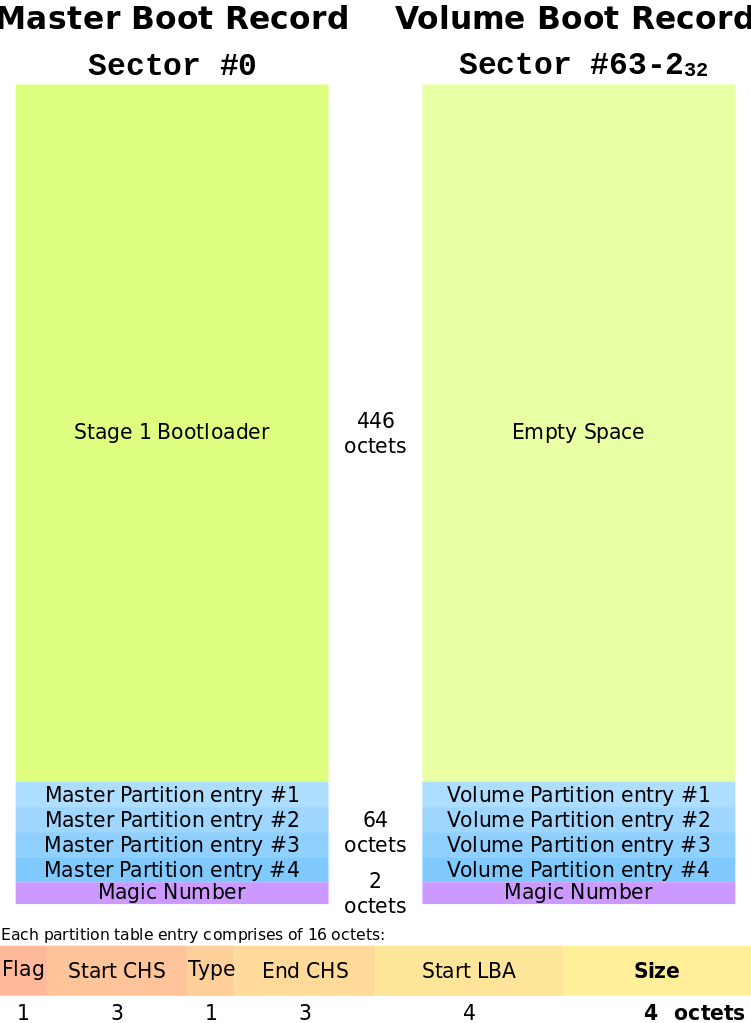
\includegraphics[scale=0.4]{images/mbr_layout.png}
	\caption{Grobes MBR-Layout}
	\label{fig:mbr_layout}
\end{figure}

\pagebreak{}

\begin{figure}[h]
	\centering
	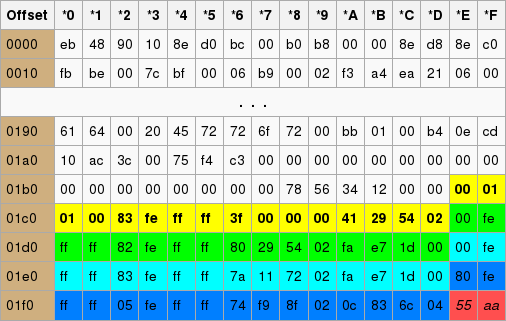
\includegraphics[scale=0.6]{images/partitionstabelle.png}
	\caption{Position der Partitionstabelle}
	\label{fig:mbr_parttab}
\end{figure}

\begin{table}[h]
	\begin{center}
		\begin{tabular}[c]{ | l | l | l |}
		\hline
		\cellcolor{grey} Offset & \cellcolor{grey} Inhalt & \cellcolor{grey} Größe in Bytes \\ \hline
		0x00 & Bootfähigkeit \(0x80_{hex}=bootable, 0x00_{hex}=not bootable\) & 1\\ \hline
		0x01 & CHS-Eintrag des ersten Sektors & 3 \\ \hline
		0x04 & Partitionstyp & 1 \\ \hline
		0x05 & CHS-Eintrag des letzten Sektors & 3 \\ \hline
		0x08 & Startblock (gezählt ab 0 = Plattenanfang) & 4 \\ \hline
		0x0C & Anzahl der Blöcke (LBA-Nummerierung, je 512 Bytes) & 4\\ \hline
		\end{tabular}
	\end{center}
	
	\caption{Aufbau eines Partitionstabelleneintrags (Offset bezieht sich auf den Anfang eines Partitionstabelleneintrages)}
	\label{tab:mbr_partentry_tbl}
\end{table}

\pagebreak{}

\begin{table}[h]
	\begin{center}
		\begin{tabular}[c]{ | l | l |}
		\hline
		\cellcolor{grey} Typcode & \cellcolor{grey} Bezeichner \\ \hline
		0x00 & leer/unbenutzt \\ \hline
		0x06 & FAT16 \(>\) 32 MiB \\ \hline
		0x07 & NTFS (Windows NT/2000/XP/Vista/7/8), HPFS (OS/2) oder exFAT \\ \hline
		0x0B & FAT32 \\ \hline
		0x82 & Linux Swap / Solaris 2.6 X86 bis Solaris 9 X86 \\ \hline
		0x83 & Linux Native \\ \hline
		0xA6 & OpenBSD \\ \hline
		\end{tabular}
	\end{center}
	
	\caption{Auswahl einiger Partitionstypen und deren Kodierung}
	\label{tab:mbr_parttype}
\end{table}

\begin{figure}[h]
	\centering
	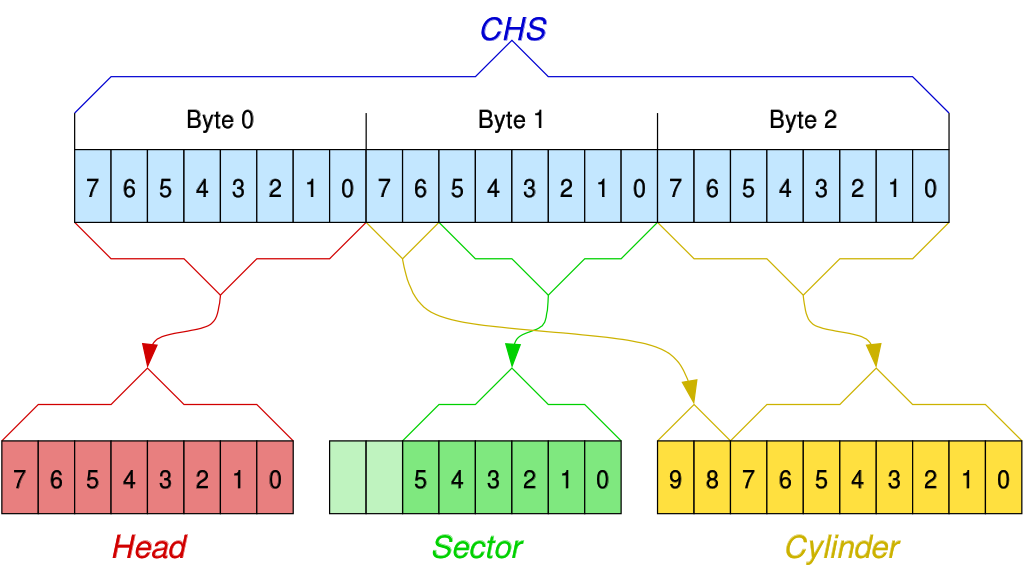
\includegraphics[scale=0.3]{images/chs_entry.png}
	\caption{Aufbau eines CHS-Eintrags}
	\label{fig:mbr_chsentry}
\end{figure}

\subsection{Beispielhafter Aufbau eines CHS-Eintrags}
\paragraph{Fragestellung}
Angenommen die folgenden Bytes liegen der Reihe nach
im MBR: 0xF3 0xFF 0x32. Bestimmen Sie die Nummer des Kopfs, des
Sectors und des Zylinders. 
\paragraph{Lösung}
\begin{itemize}
	\item Kopf: \(F3_{(16)} = 243_{(10)}\),
	\item Sektor: \(FF_{(16)} = 1111111_{(2)} \Rightarrow 00111111_{(2)} = 127_{(10)}\) 
	\item Zylinder: \(FF_{(16)}, 32_{(16)} \Rightarrow 1100000000_{(2)} + 32_{(16)} = 50_{(10)} + 512_{(10)} + 256_{(10)} = 818_{(10)}\)
\end{itemize}
\pagebreak{}

\subsection{Kontext des MBRs in einem PC-System}
\begin{figure}[h]
	\caption{Partitionslayout}
	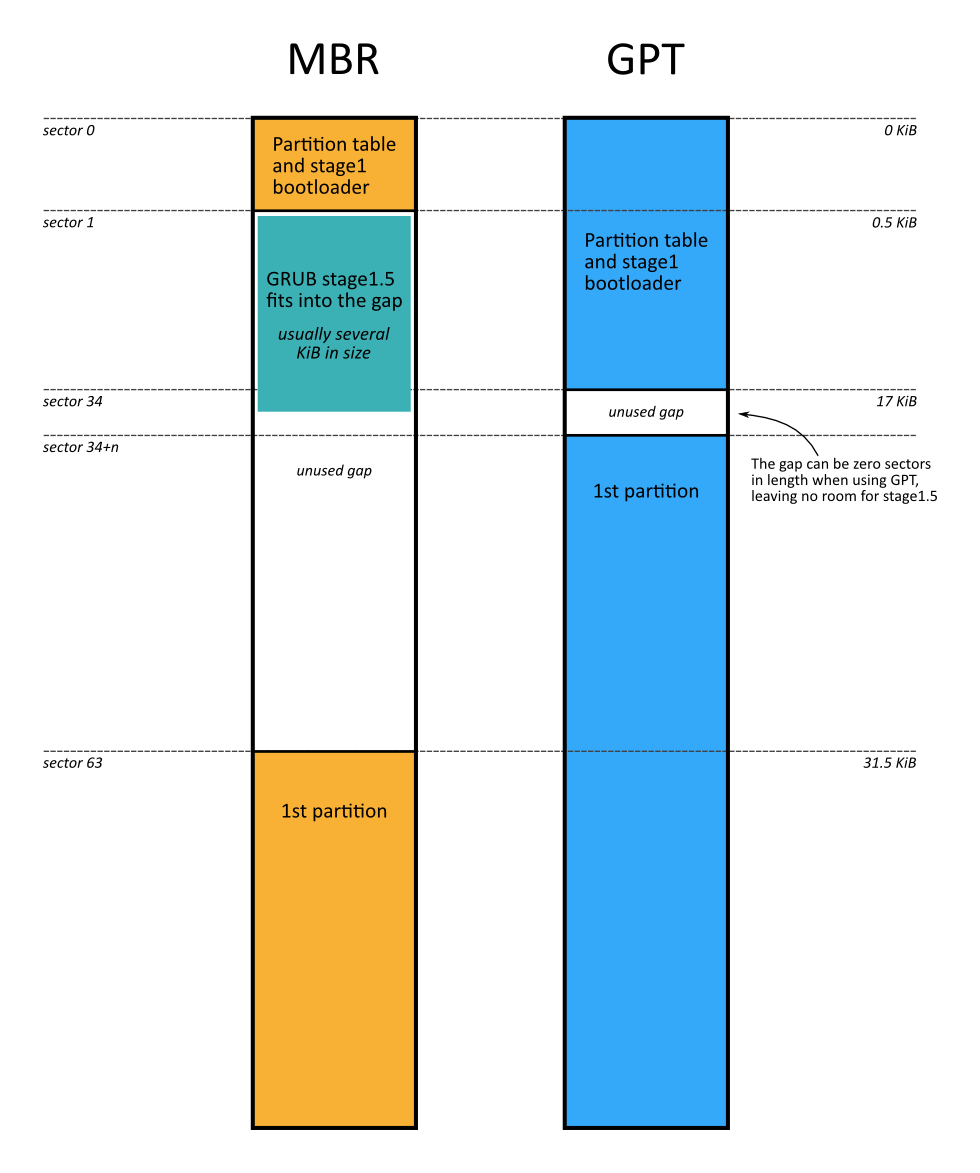
\includegraphics[scale=0.78]{images/mbr_partition_layout.png}
	\label{fig:part_layout}
\end{figure}

\pagebreak{}

\section{Übung}
\begin{enumerate}
	\item Geben Sie den gesamten MBR einer Festplatte mittels \inlinebash$dd$ und 
		\inlinebash$hexdump$ aus.
	\item Geben Sie den Partitionstabelleneintrag der ersten Partition aus. Hinweis:
		Verwenden Sie wieder \inlinebash$dd$ und \inlinebash$hexdump$
	\item Bestimmen Sie:
		\begin{itemize}
			\item den Typ der Partition,
			\item den Start-CHS-Eintrag (Welche Nummer hat der Zylinder?),
			\item die Startfähigkeit der Partition,
			\item die Anzahl der Sektoren,
			\item den End-CHS-Eintrag (Welche Nummer hat der Kopf?) und
			\item den Startsektor.
		\end{itemize}
		Hinweis: Die Felder der Partitionstabelleneinträge werden immer im 
			Little-Endian-Format abgespeichert

	\item Welches Problem sehen Sie im Bezug auf Partitionstabelleneinträge (LBA) im Zusammenhang
		mit Partitionsgrößen?
\end{enumerate}
\end{document}
